\documentclass[11pt,a4paper]{article}
%\documentclass[11pt,a4paper]{scrartcl}
%\documentclass[11pt,a4paper,oneside]{book}
\usepackage[british,UKenglish,USenglish,english,american]{babel}
%\usepackage[a4paper, total={16cm, 23cm}]{geometry}
\usepackage[tmargin = 1.25in,bmargin = 1.25in,lmargin = 1in,rmargin = 
1in]{geometry}
\usepackage{tikz}
\usepackage{graphicx}
\usepackage{pgfplots}
\pgfplotsset{width=12cm,compat=1.9}

\usepackage{chemmacros}
\usepackage{chemfig}
%\usepackage{ghsystem}
\usechemmodule{redox}
%\usepackage{chemnum}
%\usepackage{bohr}
%\usepackage{elements}
%\usepackage{endiagram}
%\usepackage{modiagram}
%\usepackage{chemgreek}
\usepackage{mhchem}
\usepackage{esint}
\usepackage{tabularray}

\usepackage{makeidx}
\usepackage{epstopdf}

\usepackage{amssymb}
\usepackage{mathrsfs}
%\usepackage{minted}
\usepackage{bm}
\usepackage{amsmath}
\usepackage{enumitem}
\usepackage[english]{varioref}
\usepackage[english]{babel}
\usepackage{lipsum}
\usepackage{fancyhdr}
\pagestyle{fancy} 
\usepackage{float}
\usepackage{empheq}
\usepackage[framemethod=tikz]{mdframed}
\usepackage{epstopdf}
\numberwithin{equation}{section}
\usepackage{eso-pic}
\usepackage{calc}
\usepackage{nccmath}
\usepackage{caption}
\usepackage{subcaption}
\usepackage{gensymb}
\usepackage{amsfonts,amsthm,epsfig,epstopdf,titling,url,array}
\usepackage{siunitx}
\sisetup{input-digits = 0123456789\pi}
\usepackage[symbol]{footmisc}
\usepackage{xcolor}
\usepackage{multicol}
\usepackage{boondox-cal}
\DeclareSIUnit\atm{atm}
\setcounter{secnumdepth}{3}
\setcounter{tocdepth}{3}
\usepackage{booktabs}


\DeclareSIUnit\atm{atm}

\pagestyle{fancy} 
\fancypagestyle{firstpage}{
	\rhead{\begin{picture}(0,0) 
			\put(-30,0){
\includegraphics[width=1cm]{figures/MCI_4C_bw.eps}} 
	\end{picture}}
}
\fancyhead[L]{\slshape\nouppercase{\leftmark}}
\chead{}
\rhead{\begin{picture}(0,0) 
		\put(-30,0){
\includegraphics[width=1cm]{figures/MCI_4C_bw.eps}} \end{picture}}
\lfoot{\textit{}}
\cfoot{-\ \thepage\ -}
\rfoot{\textit{}}

\DeclareMathOperator{\rank}{rank}
\DeclareMathOperator{\atantwo}{atan2}

\renewcommand{\headrulewidth}{0.4pt}
\renewcommand{\footrulewidth}{0.4pt}
\newcommand{\abs}[1]{\left|#1\right|}
\definecolor{mycolor1}{rgb}{0.97, 0.97, 0.97}
\definecolor{mycolor2}{rgb}{0.97, 0.97, 0.97}
\definecolor{tableShade}{gray}{0.9}
\newcommand{\sign}{\text{sign}}
\newcommand{\centered}[1]{\begin{tabular}{@{}l@{}} #1 \end{tabular}}
\theoremstyle{it}
\newtheorem{defn}{Definition}[section]
\newtheorem{thm}{Theorem}[section]
\newtheorem{lemma}{Lemma}[section]
\theoremstyle{definition}
%\theoremstyle{it}
\newtheorem{example}{Example}[section]

\newenvironment{myitemize_1}
{ \begin{itemize}[topsep=0pt]
		\setlength{\topsep}{2pt}		
		\setlength{\itemsep}{2pt}
		\setlength{\parskip}{2pt}
		\setlength{\parsep}{2pt}     }
	{ \end{itemize}                  }


\newmdenv[innerlinewidth=0.5pt, roundcorner=4pt,backgroundcolor=mycolor2, 
linecolor=mycolor1,innerleftmargin=6pt,
innerrightmargin=6pt,innertopmargin=6pt,innerbottommargin=6pt]{mybox}

\title{\textbf{LRCL modelization}}
\author{\textbf{dab@mci4me.at}}

\begin{document}
	\thispagestyle{firstpage}
	\begin{mybox}
		\maketitle
		\vspace{125mm}
	\end{mybox}
	\newpage
	\tableofcontents
	\listoffigures	
	\listoftables
	\newpage

\section{Model description}

\begin{figure}[H]
	\centering
		\includegraphics[width = 300pt, angle = 0, 
		keepaspectratio]{figures/electric_schematic_LRCL_filter_2.eps}
		\captionsetup{width=0.5\textwidth}	
		\caption{LRCL electrical schematic.}
	\label{lrcl_fig1}
\end{figure}

\noindent\textbf{Kirchhoff's equations}\footnote[2]{Physical relation between voltage variation and relative charge variation of an electrical capacitor:
\begin{flalign*}
	CdV(t)=dQ(t)\Rightarrow C\frac{dV(t)}{dt}=i_c(t) &&
\end{flalign*}
}:
\begin{flalign}
	& u_1(t) - R_1i_1(t) - L_1\frac{di_1(t)}{dt}-u_g(t) = 0  \label{lrcl_eq_1} \\[6pt]
	& u_g(t) - R_2i_2(t) - L_2\frac{di_2(t)}{dt}-u_2(t) = 0  \label{lrcl_eq_2} \\[6pt]
	& i_1(t) - i_2(t) - i_c(t) = 0 \label{lrcl_eq_3} \\[6pt]
	& u_g(t) - R_ci_c(t) - u_c(t) = 0 \label{lrcl_eq_4} \\[6pt]
	& i_c(t) = C\frac{du_c(t)}{dt}  \label{lrcl_eq_5}
\end{flalign}
Eq.~\eqref{lrcl_eq_4} and Eq.~\eqref{lrcl_eq_3} can be merged and Eq.~\eqref{lrcl_eq_4} can be written as follows
\begin{flalign}
	& u_g(t) = R_c\Big[i_1(t)-i_2(t)\Big] + u_c(t) \label{lrcl_eq_6}
\end{flalign}
Eq.~\eqref{lrcl_eq_3} and Eq.~\eqref{lrcl_eq_4}-Eq.~\eqref{lrcl_eq_5} can be merged and can be written as follows
\begin{flalign}
	& i_c(t) = i_1(t) - i_2(t) = C\frac{du_c(t)}{dt} \label{lrcl_eq_7}
\end{flalign}
Combining Eq.~\eqref{lrcl_eq_6}-Eq.~\eqref{lrcl_eq_7} with Eq.~\eqref{lrcl_eq_1}-Eq.~\eqref{lrcl_eq_2} we obtain the following system
\begin{flalign}
	& u_1(t) - R_1i_1(t) - L_1\frac{di_1(t)}{dt}-\Big\{R_c\Big[i_1(t)-i_2(t)\Big] + u_c(t)\Big\} = 0  \\[6pt]
	& R_c\Big[i_1(t)-i_2(t)\Big] + u_c(t) - R_2i_2(t) - L_2\frac{di_2(t)}{dt}-u_2(t) = 0  \\[6pt]
	& C\frac{du_c(t)}{dt} = i_1(t) - i_2(t)
\end{flalign}
or 
\begin{flalign}
	& L_1\frac{di_1(t)}{dt} = - \Big(R_1 + R_c\Big)i_1(t) + R_ci_2(t) - u_c(t) + u_1(t) \\[6pt]
	& L_2\frac{di_2(t)}{dt} = R_ci_1(t) - \Big(R_2 + R_c\Big)i_2(t) + u_c(t) - u_2(t) \\[6pt]
	& C\frac{du_c(t)}{dt} = i_1(t) - i_2(t)
\end{flalign}
and 
\begin{flalign}
	& \frac{di_1(t)}{dt} = - \frac{R_1 + R_c}{L_1}i_1(t) + \frac{R_c}{L_1}i_2(t) - \frac{1}{L_1}u_c(t) + \frac{1}{L_1}u_1(t)  \label{lrcl_eq_8} \\[6pt]
	& \frac{di_2(t)}{dt} = \frac{R_c}{L_2}i_1(t) - \frac{R_2 + R_c}{L_2}i_2(t) + \frac{1}{L_2}u_c(t) - \frac{1}{L_2}u_2(t)  \label{lrcl_eq_9} \\[6pt]
	& \frac{du_c(t)}{dt} = \frac{1}{C}\Big[i_1(t) - i_2(t)\Big] \label{lrcl_eq_10}
\end{flalign}
To write the system of Eq.~\eqref{lrcl_eq_8}-Eq.~\eqref{lrcl_eq_10} in a state space form it is necessary to define the input and the output of the system as follows
\begin{flalign}
	& u(t) = u_1(t)  \label{lrcl_eq_11} \qquad \textit{this is the input (scalar) of the system}\\[6pt]
	& \vec{y}(t) = \begin{bmatrix} i_1(t) \\ i_2(t) \\ u_g(t) \end{bmatrix} \label{lrcl_eq_12} \qquad \textit{this is the output (vector) of the system}
\end{flalign}
the system contains also another term $u_2(t)$ which can be treated as a unknown (or partially unknown)  disturbance.

Obviously the state vector is represented by the vector
\begin{flalign}
	& \vec{x} =  \begin{bmatrix} i_1(t) \\ i_2(t) \\ u_c(t) \end{bmatrix} \label{lrcl_eq_13}
\end{flalign}

The system Eq.~\eqref{lrcl_eq_8}-Eq.~\eqref{lrcl_eq_10} can be now written in a matrix form as follows
\begin{flalign}
	& \dot{\vec{x}}(t) =  \tilde{\mathbf{A}}\vec{x}(t) + \tilde{\mathbf{B}}u_1(t) + \tilde{\mathbf{E}}u_2(t) \label{lrcl_eq_14} \\[6pt]
	& {\vec{y}}(t) =  \mathbf{C}\vec{x}(t) \label{lrcl_eq_15}
\end{flalign}
where
\begin{flalign}
	& \tilde{\mathbf{A}} =  
	\begin{bmatrix}
		 -\frac{R_1 + R_c}{L_1} & \frac{R_c}{L_1} & -\frac{1}{L_1} \\[6pt]
		 \frac{R_c}{L_2} & -\frac{R_2+R_c}{L_2} & \frac{1}{L_2} \\[6pt]
		 \frac{1}{C} & -\frac{1}{C} & 0
	 \end{bmatrix} \label{lrcl_eq_16}
\end{flalign}
\begin{flalign}
	& \tilde{\mathbf{B}} =  
	\begin{bmatrix}
		\frac{1}{L_1} \\[6pt]
		0 \\[6pt]
		0
	\end{bmatrix} \qquad
	\tilde{\mathbf{E}} =  
	\begin{bmatrix}
		0 \\[6pt]
		-\frac{1}{L_2} \\[6pt]
		0
	\end{bmatrix}
\label{lrcl_eq_18}
\end{flalign}
and 
\begin{flalign}
	& \mathbf{C} =  
	\begin{bmatrix}
		1 & 0 & 0 \\[6pt]
		0 & 1 & 0 \\[6pt]
		R_c & -R_c & 1
	\end{bmatrix} =  
	\begin{bmatrix}
		\mathbf{C}_1 \\[6pt]
		\mathbf{C}_2 \\[6pt]
		\mathbf{C}_3
	\end{bmatrix}
	\label{lrcl_eq_19}
\end{flalign}

The transfer function between the input $u_1(t)$ and the output $u_g(t)$ can be represented as follows
\begin{flalign}
	& H_g(s) = \frac{U_g(s)}{U_1(s)} = \mathbf{C}_3\Big[s\mathbf{I}_3-\tilde{\mathbf{A}}\Big]^{-1}\tilde{\mathbf{B}} \label{lrcl_eq_20}
\end{flalign}
and result is in the form
\begin{flalign}
	& H_g(s) = \frac{b_2s^2+b_1s+b_0}{s^3+a_2s^2+a_1s+a_0} \label{lrcl_eq_21}
\end{flalign}

The transfer function between the input $u_1(t)$ and the output $i_2(t)$ can be represented as follows
\begin{flalign}
	& H_2(s) = \frac{I_2(s)}{U_1(s)} = \mathbf{C}_2\Big[s\mathbf{I}_3-\tilde{\mathbf{A}}\Big]^{-1}\tilde{\mathbf{B}} \label{lrcl_eq_22}
\end{flalign}
and result is in the form
\begin{flalign}
	& H_2(s) = \frac{b_1s+b_0}{s^3+a_2s^2+a_1s+a_0} \label{lrcl_eq_23}
\end{flalign}

The transfer function between the input $u_1(t)$ and the output $i_1(t)$ can be represented as follows
\begin{flalign}
	& H_1(s) = \frac{I_1(s)}{U_1(s)} = \mathbf{C}_1\Big[s\mathbf{I}_3-\tilde{\mathbf{A}}\Big]^{-1}\tilde{\mathbf{B}} \label{lrcl_eq_24}
\end{flalign}
and result is in the form
\begin{flalign}
	& H_1(s) = \frac{b_2s^2+b_1s+b_0}{s^3+a_2s^2+a_1s+a_0} \label{lrcl_eq_25}
\end{flalign}

In the following, the $H_2(s)$ transfer function of Eq.~\eqref{lrcl_eq_23} will be taken into account. This transfer function is derived from the state space system
\begin{flalign}
	& \dot{\vec{x}}(t) =  \tilde{\mathbf{A}}\vec{x}(t) + \tilde{\mathbf{B}}u_1(t) \\[6pt]
	& i_2(t) =  \mathbf{C}_2\vec{x}(t)  
\end{flalign} 
where the disturbance term $u_2(t)$ has been omitted. \\


The coefficients relative to Eq.~\eqref{lrcl_eq_23} are as follows
\begin{flalign}
	& a_2 = \frac{L_1R_c+L_2R_c+L_1R_2+L_2R_1}{L_1L_2} \label{lrcl_eq_26} \\[6pt]
	& a_1 = \frac{L_1+L_2+R_2R_cC+R_1R_2C+R_1R_2C}{L_1L_2C} \label{lrcl_eq_27} \\[6pt]
	& a_0 = \frac{R_1+R_2}{L_1L_2C} \label{lrcl_eq_28} \\[6pt]
	& b_1 = \frac{R_c}{L_1L_2} \label{lrcl_eq_29} \\[6pt]
	& b_0 = \frac{1}{L_1L_2C} \label{lrcl_eq_30}
\end{flalign}
The transfer function of Eq.~\eqref{lrcl_eq_23} can be rewritten in state space form using the controllable canonical form as follows
\begin{flalign}
	& \dot{\vec{z}}(t) =  \tilde{\mathbf{M}}\vec{z}(t) + \tilde{\mathbf{N}}u_1(t) \label{lrcl_eq_31} \\[6pt]
	& {y}(t) =  i_2(t) = \mathbf{G}\vec{z}(t)  \label{lrcl_eq_32}
\end{flalign}
where
\begin{flalign}
	& \tilde{\mathbf{M}} = \begin{bmatrix}
		0&1&0 \\ 0&0&1 \\ -a_0&-a_1&-a_2
	\end{bmatrix}, \quad
	\tilde{\mathbf{N}} = \begin{bmatrix}
	0 \\ 0 \\ 1
\end{bmatrix} \label{lrcl_eq_33}
\end{flalign}
and 
\begin{flalign}
	& \mathbf{G} = \begin{bmatrix}
		b_0 & b_1 & 0
	\end{bmatrix} \label{lrcl_eq_34}
\end{flalign}



\begin{flalign}
	&	i_2^{(0)}(t) = \mathbf{G}\vec{z}(t) \label{lrcl_eq_35} \\[6pt]
	&	i_2^{(1)}(t) = \mathbf{G}\tilde{\mathbf{M}}\vec{z}(t) + \mathbf{G}\tilde{\mathbf{N}}u_1(t) \label{lrcl_eq_36} \\[6pt]
	&	i_2^{(2)}(t) = \mathbf{G}\tilde{\mathbf{M}}^2\vec{z}(t) + \mathbf{G}\tilde{\mathbf{M}} \tilde{\mathbf{N}}u_1(t) \label{lrcl_eq_37}
\end{flalign}













\end{document} 